\documentclass[11pt,spanish]{article}
\usepackage[utf8]{inputenc}
\usepackage{float}
\usepackage{siunitx}

%Packages del style de Nico
\usepackage[T1]{fontenc}
\usepackage[spanish]{babel}
\usepackage{geometry}
\geometry{verbose,tmargin=2cm,bmargin=2cm,lmargin=2cm,rmargin=2cm}
\usepackage{amssymb}
\usepackage{amstext}
\usepackage{amsmath}
\usepackage{graphicx}
\usepackage{listings}


\usepackage{xcolor}

%New colors defined below
\definecolor{codegreen}{rgb}{0,0.6,0}
\definecolor{codegray}{rgb}{0.5,0.5,0.5}
\definecolor{codepurple}{rgb}{0.58,0,0.82}
\definecolor{backcolour}{rgb}{0.95,0.95,0.92}

%Code listing style named "mystyle"
\lstdefinestyle{mystyle}{
  backgroundcolor=\color{backcolour}, commentstyle=\color{codegreen},
  keywordstyle=\color{magenta},
  numberstyle=\tiny\color{codegray},
  stringstyle=\color{codepurple},
  basicstyle=\ttfamily\footnotesize,
  breakatwhitespace=false,         
  breaklines=true,                 
  captionpos=b,                    
  keepspaces=true,                 
  numbers=left,                    
  numbersep=5pt,                  
  showspaces=false,                
  showstringspaces=false,
  showtabs=false,                  
  tabsize=2
}

%"mystyle" code listing set
\lstset{style=mystyle}
%\usepackage[numbers]{natbib}
%\setlength{\bibsep}{0.0pt}
\usepackage[auth-sc]{authblk}
\usepackage{hyperref}
\usepackage{notoccite}
\usepackage{fancyhdr}
\usepackage[font=small,labelfont=bf]{caption}
\usepackage{xspace}
\usepackage{xcolor}
\usepackage[largesc,theoremfont]{newpxtext}
\usepackage{multirow}
\usepackage{booktabs}
%\usepackage[switch*,modulo]{lineno}
%\linenumbers
\usepackage{cleveref}
\usepackage{todonotes}
\usepackage{mathtools}
\usepackage{subfigure}

\pagestyle{fancy}
\lhead{}
\rhead{Practia escuela }

\begin{document}

\renewcommand\Authfont{\fontsize{12}{14.4}\selectfont}
\renewcommand\Affilfont{\fontsize{9}{10.8}\itshape}
\renewcommand\Authand{,}
\renewcommand\Authands{,}

\title{Predicción de ventas de hamburguesas Krustyburger}

\author[1]{Alexis~Pacek}


\affil[1]{\footnotesize Practia Global, Buenos Aires, Argentina}

\date{Octubre 2021}

\maketitle

\begin{abstract}


\end{abstract}

\section{Exploración de los datos}
En esta etapa buscamos entender cuales son las características del dataset.
Para dicho fin se procede respondiendo ciertas preguntas básicas utilizando Jupyter Notebook.

\vspace{3mm}

\textbf{¿Qué features contiene el dataset?}

\vspace{3mm}

Utilizando la librería \textit{pandas} vemos que el dataset esta conformado por 5 columnas y 5170352 filas, donde las columnas representan los atributos (features) y las filas son las muestras.
En la \cref{fig:head} se muestran las primeras 5 filas del dataset con sus correspondientes atributos.

\begin{figure}[H]
    \centering
    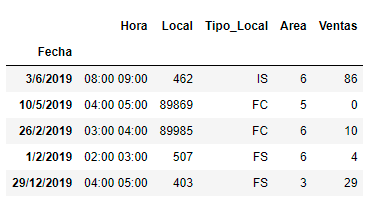
\includegraphics{Exploratorio/head.png}
    \caption{Las columnas son los atributos y las filas son los datos. Se muestran solo las primeras 5 filas.}
    \label{fig:head}
\end{figure}

Entonces vemos que cada entrada del dataset tendría que tener asignado \textit{Fecha}, ventana temporal (\textit{Hora}), número de local (\textit{Local}), tipo de local (\textit{Tipo\_Local}), número de área (\textit{Area}) y cantidad de ventas de hamburguesas (\textit{Ventas}).

\vspace{3mm}

\textbf{¿La tabla posee valores nulos?}

\vspace{3mm}

Los valores nulos con este dataset podrían ser de tipo: \textit{NaN}, \textit{None} y \textit{Empy string}.

Utilizando el \cref{empys} se obtiene la suma total de strings vacíos en el dataset. 
\vspace{2mm}
\begin{lstlisting}[language=Python, caption= Código para encontrar la cantidad de stings vacios, label = empys]
DataFrame.applymap(lambda x: x == '').sum().sum()

\end{lstlisting}
\vspace{2mm}

Básicamente lo que hace el código es un mapeado \cite{applymap} a todo el dataset con booleanos, donde se obtiene \textit{True} en los lugares donde hay un string vacio y luego con el .sum().sum() consigo sumar todos los \textit{True} hallados. Entonces consecuentemente se encuentra la cantidad de entradas con strings vacíos.

Por otro lado para contabilizar los \textit{NaN} y \textit{None} utilizo. 

\vspace{2mm}
\begin{lstlisting}[language=Python, caption= Codigo para encontrar la cantidad de \textit{NaN} y \textit{None}. , label=nan]
DataFrame.isnull().sum().sum()

\end{lstlisting}
\vspace{2mm}

En el \cref{nan} se usó isnull() \cite{isnull} que es una función de pandas con el objetivo especifico de hacer un mapeo booleano, igual que antes, pero ahora los True para los \textit{Nan} o \textit{None}].

\vspace{3mm}
En ambos casos se obtiene que el dataset esta libre de valores nulos.

\vspace{3mm}

\textbf{¿Cuántos locales posee la empresa?}

\vspace{3mm}


Aquí se cuentan la cantidad de elementos que hay en un array conformado por los id's de los locales sin repetir. 
Se obtuvo que hay 232 locales. 

\vspace{3mm}

\textbf{¿Cuántos tipos de locales hay?}

\vspace{3mm}

Se forma un array con todos los valores que hay en el atributo \textit{Tipo de Local} del data set y luego se descargan los valores que se repiten.
Consecuentemente se obtiene una lista de 4 tipos de locales que no se repiten. 

Ellos son:  

\begin{itemize}
    \item IS
    \item FC
    \item FS
    \item MS
\end{itemize}

\vspace{3mm}

\textbf{¿Cuántos locales hay por cada tipo?}

\vspace{3mm}

Primero se busca que efectivamente cada local tenga una única etiqueta de los cuatro tipos de locales posible. 
Para esto se emplea el \cref{unicolocal}.

\begin{lstlisting}[language=Python, caption = la variable \textbf{cantidad} indica cuantos locales tienen más de una etiqueta para el feature \textit{Tipo de local.}, label=unicolocal]
aux = []
for i in df.Local.unique():
    if len(df[df.Local==i]['Tipo_Local'].unique()) >=2:
        aux.append(len(df[df.Local==i]['Tipo_Local'].unique()))

cantidad = len(aux)

\end{lstlisting}

Para cada local se crea un array con todas las etiquetas de \textit{Tipo de Local} que tiene, luego se filtran todas las repetidas entonces si el este array contiene al menos 2 elementos se procede a guardarlo en una variable llamada auxiliar. Lo esperado es que si ningún local tiene más de dos etiquetas entonces nada se va a guardar en la variable auxiliar por lo tanto cuando calculemos el tamaño de la variable auxiliar obtendríamos cero.

Finalmente se obtiene que cada local tiene asignado un único \textit{Tipo de local}.
\vspace{2mm}
Como cada local solo esta caracterizado como uno de los 4 tipos posibles.

Filtro todas las entradas en donde se repite el número de local y cuento cuantos locales hay de cada tipo.
Se encuentra que:

\begin{itemize}
    \item 81 locales son IS (34.91\%)
    \item 37 locales son FC (15.95\%)
    \item 65 locales son FS (28.02\%)
    \item 49 locales son MS (21.12\%)
\end{itemize}

\vspace{3mm}
\textbf{¿Cuántas áreas hay?}
\vspace{3mm}

Creo un array con todos los valores de áreas que no se repiten y le calculo la longitud.

Se encuentra que hay 9 áreas.

\vspace{3mm}
\textbf{¿Todos los locales tienen la misma 
cantidad de áreas?}
\vspace{3mm}

Para hacer esto examino inicialmente 5 locales al azar y los comparo, rápidamente se encuentra que distintos locales pueden tener distintas áreas.

\vspace{3mm}

\textbf{Gráfico de la distribución de la cantidad de áreas por local.}

\vspace{3mm}

\begin{figure}[H]
    \centering
    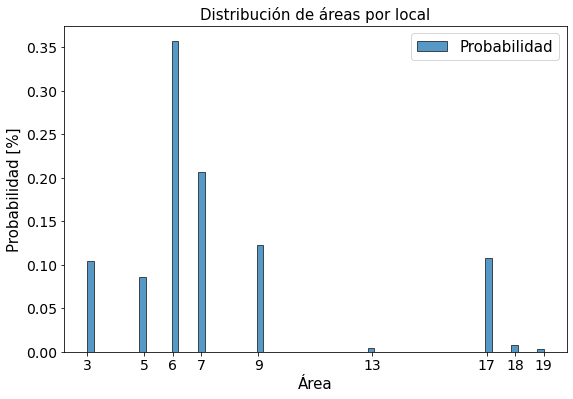
\includegraphics[width=0.8\textwidth]{Exploratorio/distribucion_area_local.png}
    \caption{Histograma normalizado con la distribución de área.}
    \label{fig:my_label}
\end{figure}
Se observa que las nueve áreas que existen están identificadas con un número y son:
\textit{3, 5, 6 ,7 ,9 13. 17, 18, 19}. Luego, la más recurrente es el área 6 que se repite el 35\% se las veces en el dataset por lo tanto es el área que más gestiones realiza (no necesariamente la que más venda).

\vspace{3mm}

\textbf{¿Están correlacionadas la hora y la venta?}

\vspace{3mm}

\section{Conclusiones}




\begin{thebibliography}{99}

\bibitem{applymap}

https://pandas.pydata.org/pandas-docs/stable/reference/api/pandas.DataFrame.applymap.html

\bibitem{isnull}
https://pandas.pydata.org/pandas-docs/stable/reference/api/pandas.isnull.html

\end{thebibliography}


\end{document}
